
\chapter{State of the Art}
This section will present a review of the literature on line simplification algorithms, stream processing algorithms and introduce several notions related to the subject of this master thesis.



\section{Moving Objects Database}
In order to maintain the location of our tracked objects, it is important to search a database for moving objects as output data for this thesis. Moving objects can be defined as objects whose value or location changes during the period under consideration. These may include vehicles, people, animals, aircraft, the air temperature in a particular city, the price of fuel at a particular filling station and the like. The widespread use of tracking devices and IoT technologies has made it possible to gather large quantities of data describing the temporal evolution of these objects and values. This opens up the possibility of designing applications using this data, which in turn leads to the need to build them \cite{MobilityDBTODS2020}.

As mentioned above the need for a specific database in order to have an efficient data storage. In the context of this thesis we will focus on MobilityDB which is a Moving Object database that extends PostgreSQL

\subsection{PostgreSQL}
PostgreSQL is an ORDBMS database management system based on POSTGRES version 4.2, developed by the Computer Science Department at the University of California at Berkeley \footnote{https://www.postgreSQL.org/docs/16/intro-whatis.html}. It is undeniable that PostgreSQL played a precursory role in the development of several concepts that were not integrated into commercial database management systems until a later date.

PostgreSQL is the open-source version derived from the original Berkeley source code, offering significant adherence to the SQL standard and providing a range of current features: complex queries, foreign keys, triggers, updatable views, transactional integrity and multi-version concurrency control.

In addition, PostgreSQL allows users to customise it in a variety of ways, such as integrating new data types, functions, operators, aggregation functions, indexing methods and procedural languages.

By virtue of its liberal licence, PostgreSQL is available to anyone to use, adapt and distribute free of charge, for any purpose, whether private, commercial or academic.

\subsection{PostGIS}
PostGIS represents a potent open-source instrument facilitating the creation of resilient spatial databases. Serving as the geographic extension of the PostgreSQL database management system, PostGIS enables the incorporation of geographic objects within data tables \cite{marquez2015PostGIS}. These geographic objects are specialized data types designed for the storage of geographic positions or sets thereof, integrated seamlessly into lines or polygons. In essence, PostGIS emerges as a formidable tool, empowering users to manage intricate geographical data proficiently and to visually interrogate such data when employed in conjunction with graphical tools, exemplified by QGIS.

\subsection{MobilityDB}
MobilityDB uses the abstract data type approach of MOD implementations \cite{guting2000foundation}. In an extensible relational database system, this is equivalent to including user-defined types that are applicable as attribute types within relations. In PostgreSQL and PostGIS, MobilityDB specifies the following temporal types: \texttt{tfloat}, \texttt{tint}, \texttt{ttext}, \texttt{tbool} , \texttt{tgeompoint} and \texttt{tgeogpoint}. These types represent functions that map from the time domain to base type domains that correspond to them. MobilityDB adds a new dimension to the existential geographical database. It responds to the need to process data about moving objects and becomes more dynamic.




\section{Line Simplification Algorithms}
Line simplification deals with the simplification of arbitrary lines, which can be straight or curved. The goal is to reduce the complexity of lines while still ensuring that the simplified representation captures the main features of the original lines. This algorithm address the problem of Line simplification this problem who is relevant for GPU computing and Spatial Data processing. The complexity of this problem is high and it is an NP-Hard problem, which makes it difficult to solve and almost impossible to obtain an optimal simplification \cite{kerkhof2022algorithmic}.

\subsection{Douglas-Peucker Algorithm}
The Douglas-Peucker algorithm  \cite{douglas1973algorithms} \cite{hershberger1994n} takes a polyline P a sequence of points $\{p_{1},..., p_{n}\}$ , and a user defined allowed spatial error, $\varepsilon$ > 0. The algorithm builds an approximation polyline $P'$ , initially consisting of $p_{1}$ and $p_{n}$. It continues adding the point pi out of the original polyline that has the largest shortest-euclidean distance to $P'$ until that distance is smaller than $\varepsilon$ as demonstrated in Figure \ref{fig:dgpk}.

\begin{figure}[!ht]
    \centering
    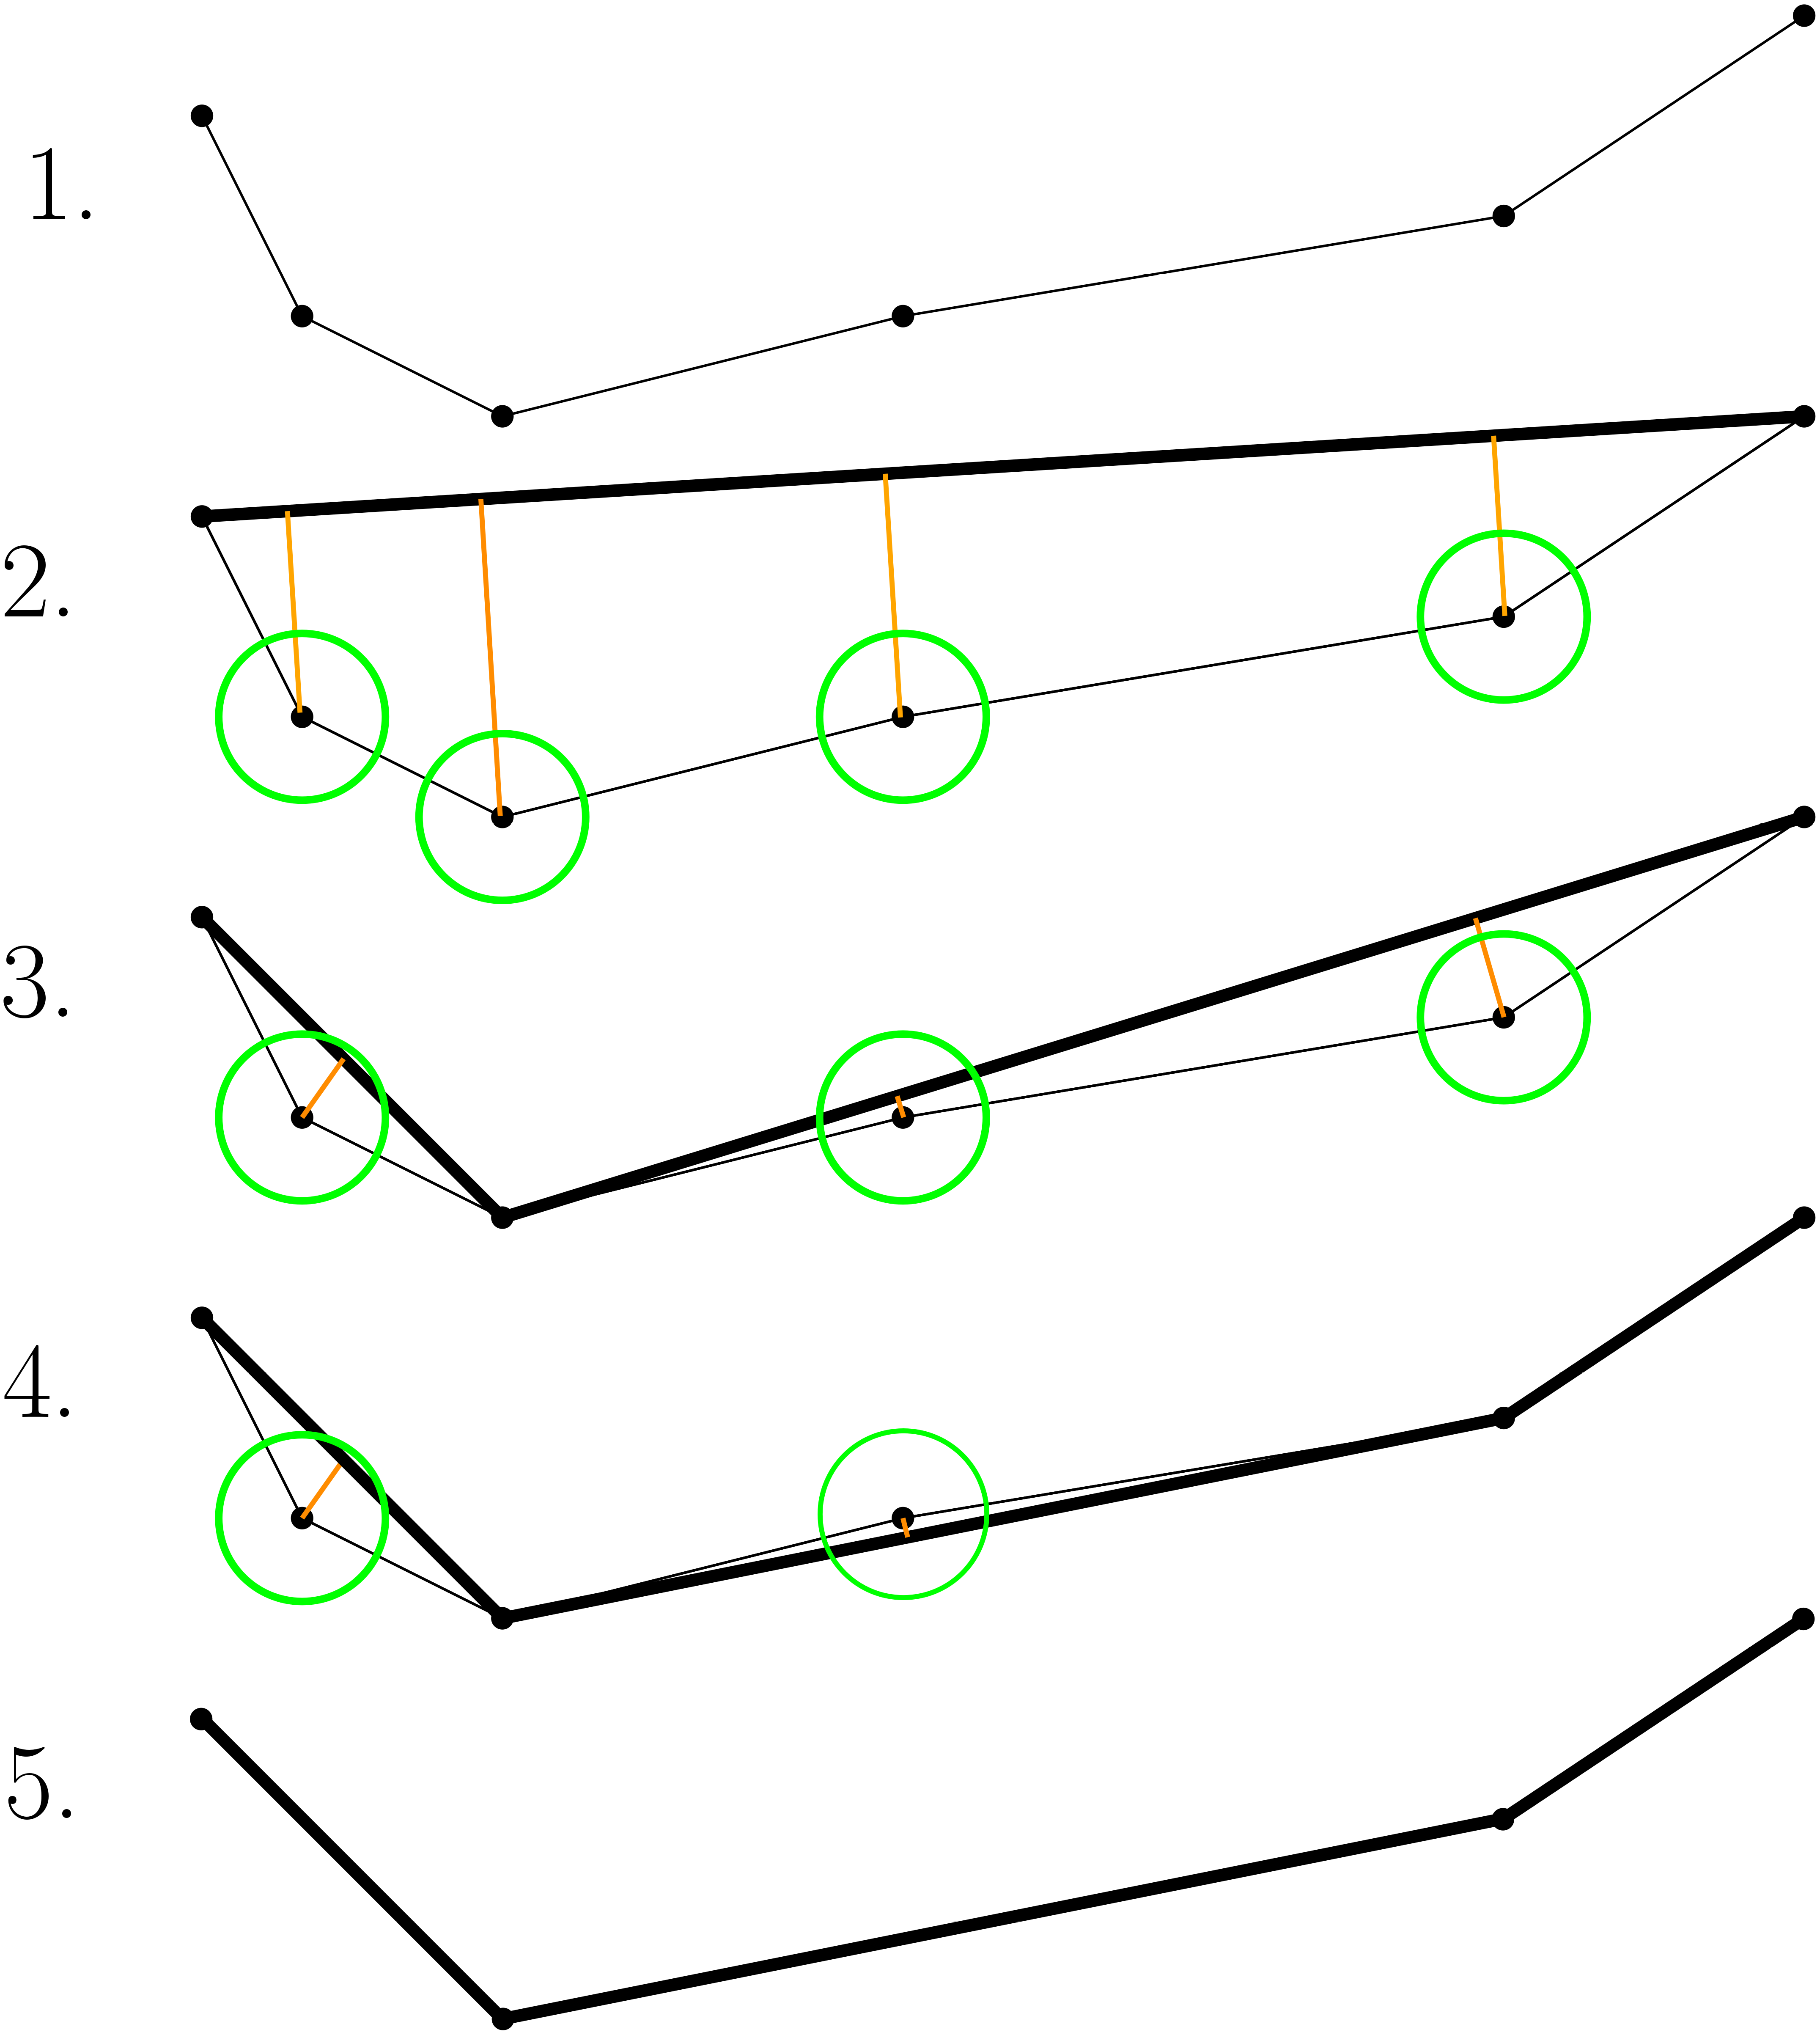
\includegraphics[width=0.5\linewidth]{figures/dgpk.png}
    \caption[Illustration of Douglas-Peucker algorithm \cite{van2017extensive}]{Illustration of how the Douglas-Peucker algorithm iteratively simplifies a line. The allowed spatial error  $\varepsilon$  is depicted with green circles \cite{van2017extensive}. }
    \label{fig:dgpk}
\end{figure}

\subsection{Minimum Distance Algorithm}
The Minimum Distance (MinDist) algorithm operates by iteratively calculating the distance between two points and retaining a point if this distance is less than the specified threshold. This algorithm is implemented in mobilitydb. It works as follows: Given a sequence of points ${p_{1},..., p_{n}}$ and a user-defined distance threshold $d > 0$, the algorithm constructs a subsequence of points $Q'$, starting with $p_{1}$. It continues adding a point $p_{i}$ to $Q'$ if the distance between $p_{i}$ and the last point added to $Q'$ is greater than or equal to $d$. This process is repeated until all points have been processed, resulting in a simplified representation of the original sequence. A temporal variant of this algorithm also exists, which considers temporal distances, ensuring that the selected points are temporally distant, making it useful for temporal data processing. 

\subsection{Visvalingam-Whyatt Algorithm}

The Visvalingam-Whyatt algorithm \cite{doi:10.1179/000870493786962263} uses the concept of ‘effective area’, which is the area of the triangle formed by a point and its two neighbors. The algorithm takes a polyline P a sequence of points $\{p_{1},..., p_{n}\}$, and a user defined allowed spatial displacement error, $\varepsilon$ > 0. For every set of three consecutive points $\{p_{i-1},p_{i},p_{i+1}\}$ a triangle is formed with its surface being the ‘effective area’. Iteratively point $p_{i}$ is dropped that results in the least areal displacement to form an approximation as illustrated in Figure \ref{fig:visv}. This process halts when the ‘effective area’ is larger than $\varepsilon$.

\begin{figure}[!ht]
    \centering
    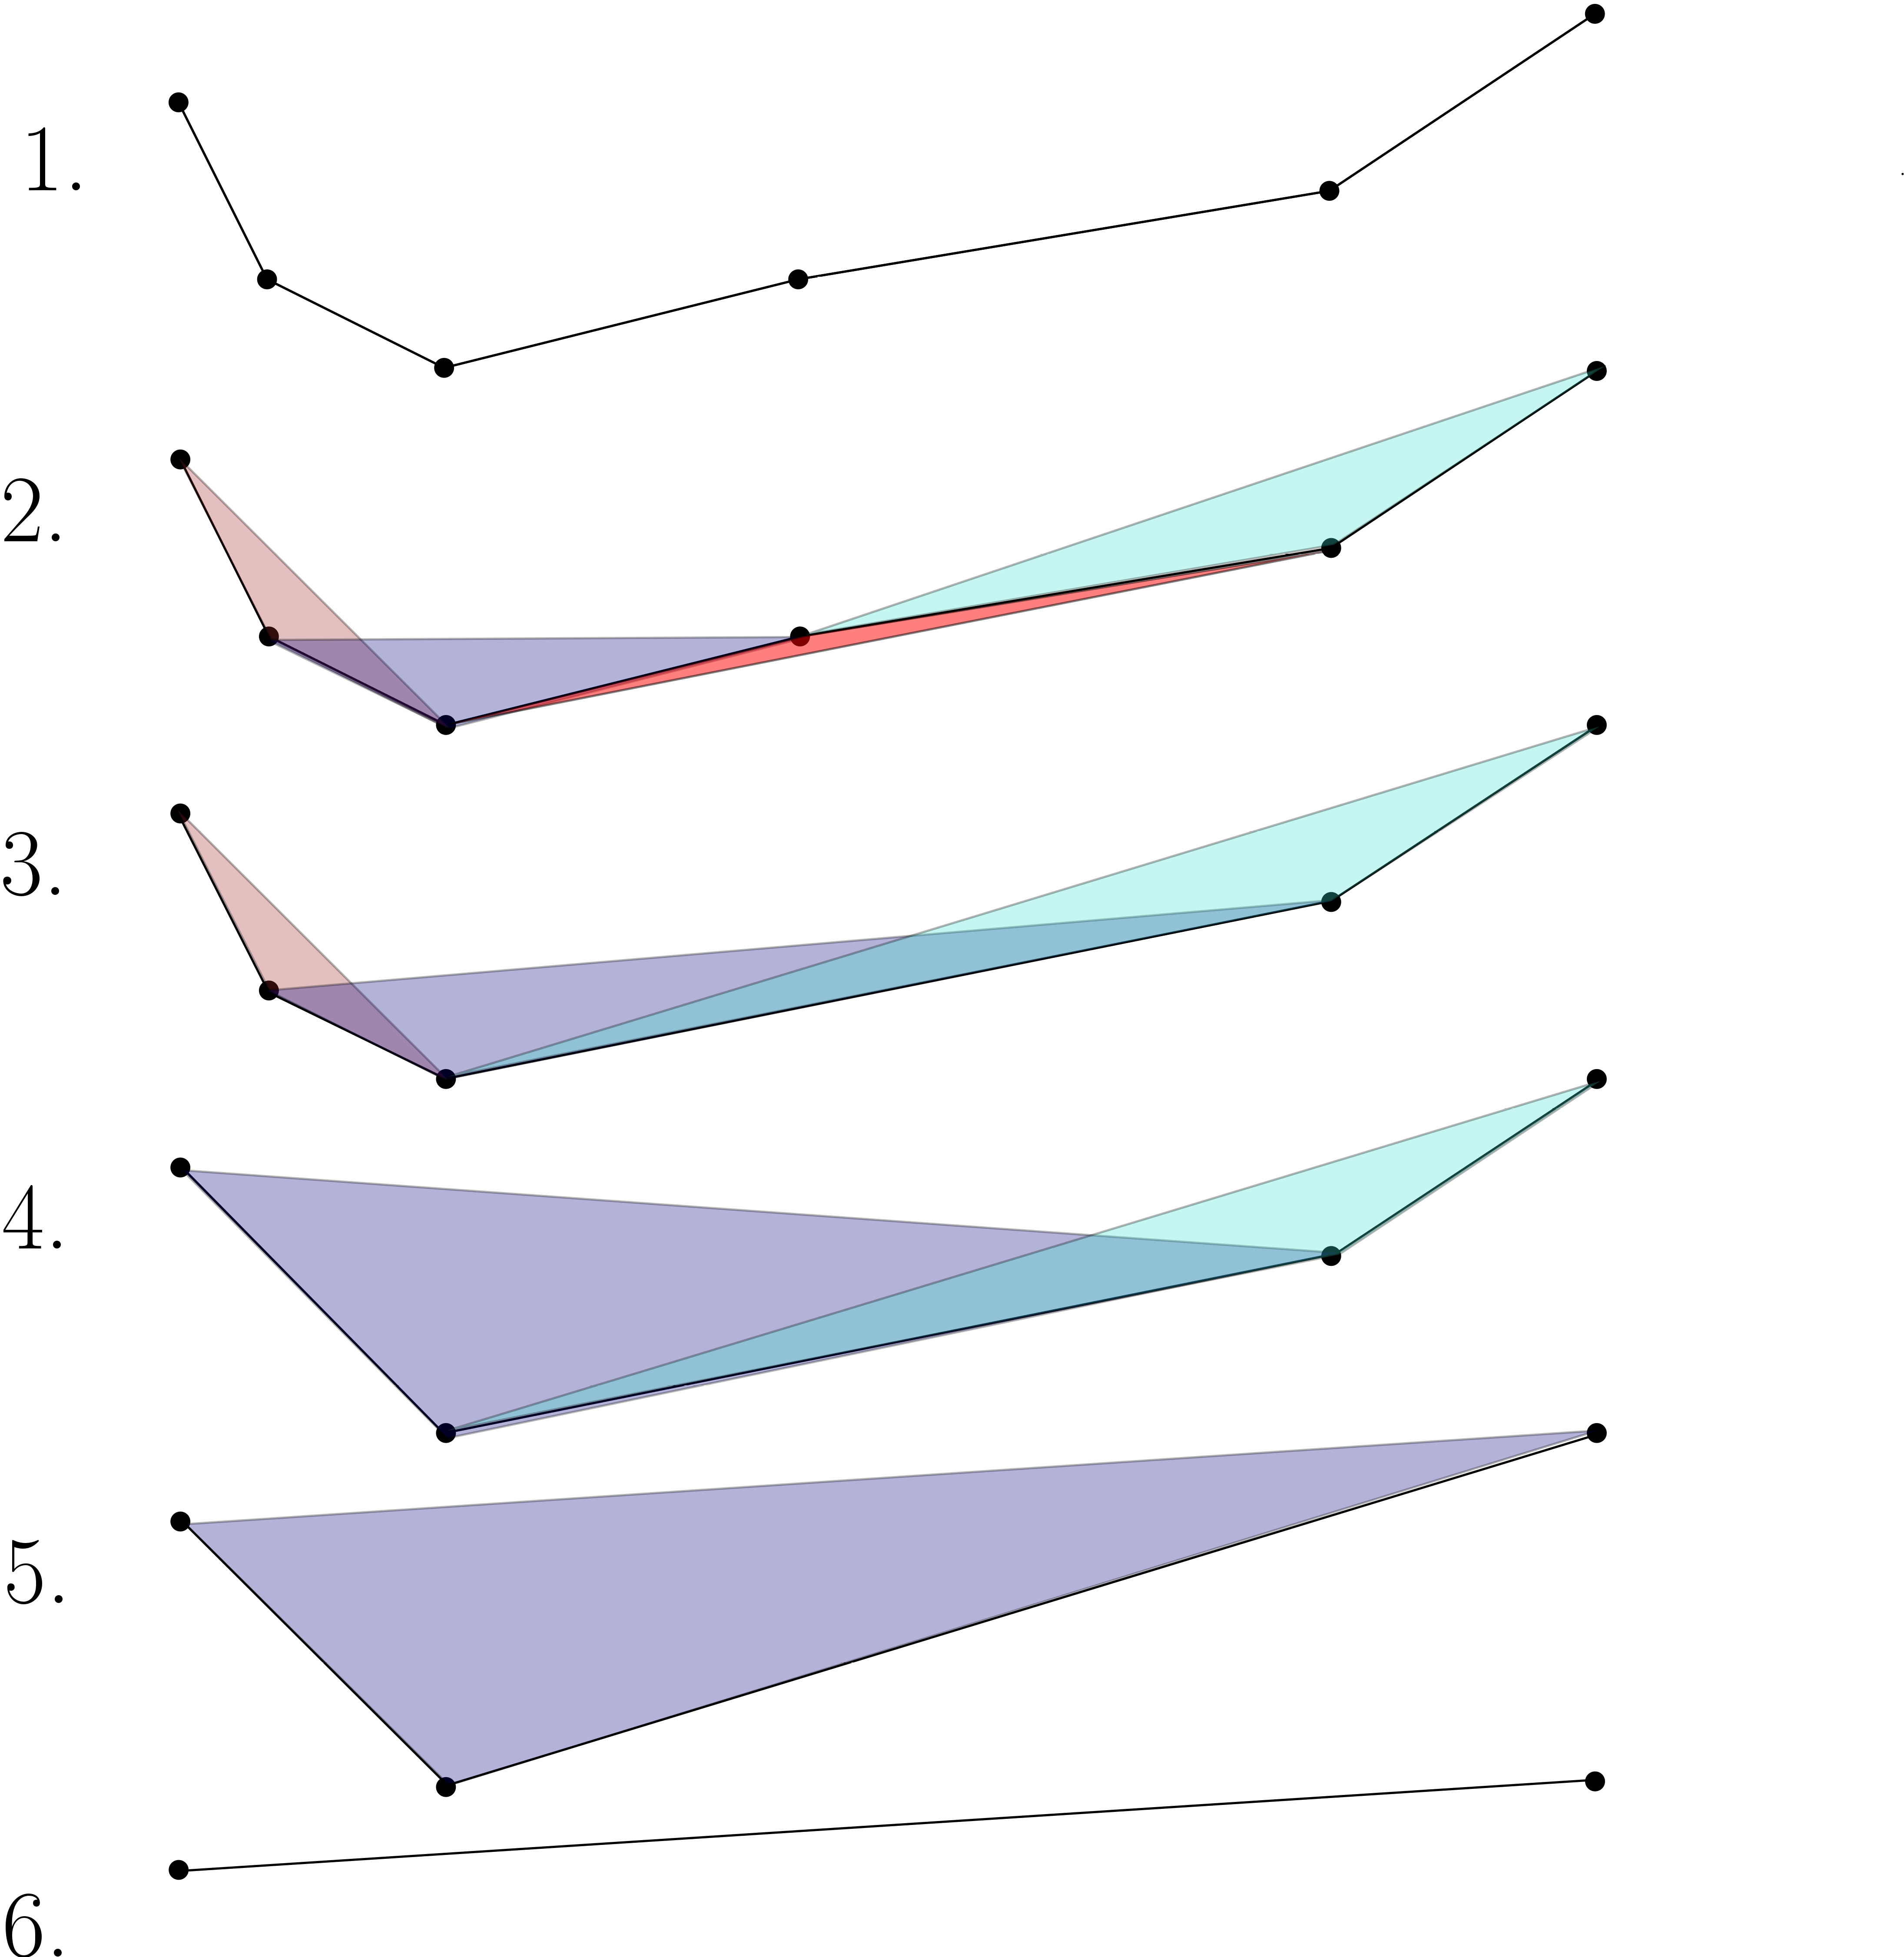
\includegraphics[width=0.5\linewidth]{figures/visv.png}
    \caption[Illustration of Visvalingam-Whyatt
    algorithm \cite{van2017extensive}.] {Illustration of Visvalingam-Whyatt
    	algorithm \cite{van2017extensive}.
    }
    \label{fig:visv}
\end{figure}

\subsection{Imai-Iri Algorithm}
The basis of the Imai-Iri algorithm \cite{IMAI198631} lies in the construction of an unweighted directed acyclic graph G. This graph is constructed by connecting all combinations of two points that would create an allowed shortcut. A breadth-first search is done on this graph to compute the shortest path connecting the first and last point, resulting in the approximation. This algorithm takes a polyline P a sequence of points $\{p_{1},..., p_{n}\}$, and a user defined allowed spatial error, $\varepsilon $ > 0. For each combination of two points ($p_{i}$ and $p_{j}$) it checks if a line between them intersects all circles with radius $\varepsilon $ that center on the points that lie{\tiny {\tiny }} between them $\{p_{x} > p_{i},p_{x} < p_{j}\}$. When this is the case, the line $p_{i}p_{j}$ is an allowed shortcut and is added to the graph G, see Figure \ref{fig:imai}. After all allowed shortcuts are added to graph G, breadth-first search is done to find the shortest path through the graph from $p_{1}$ to $p_{n}$.

\begin{figure}[!ht]
    \centering
    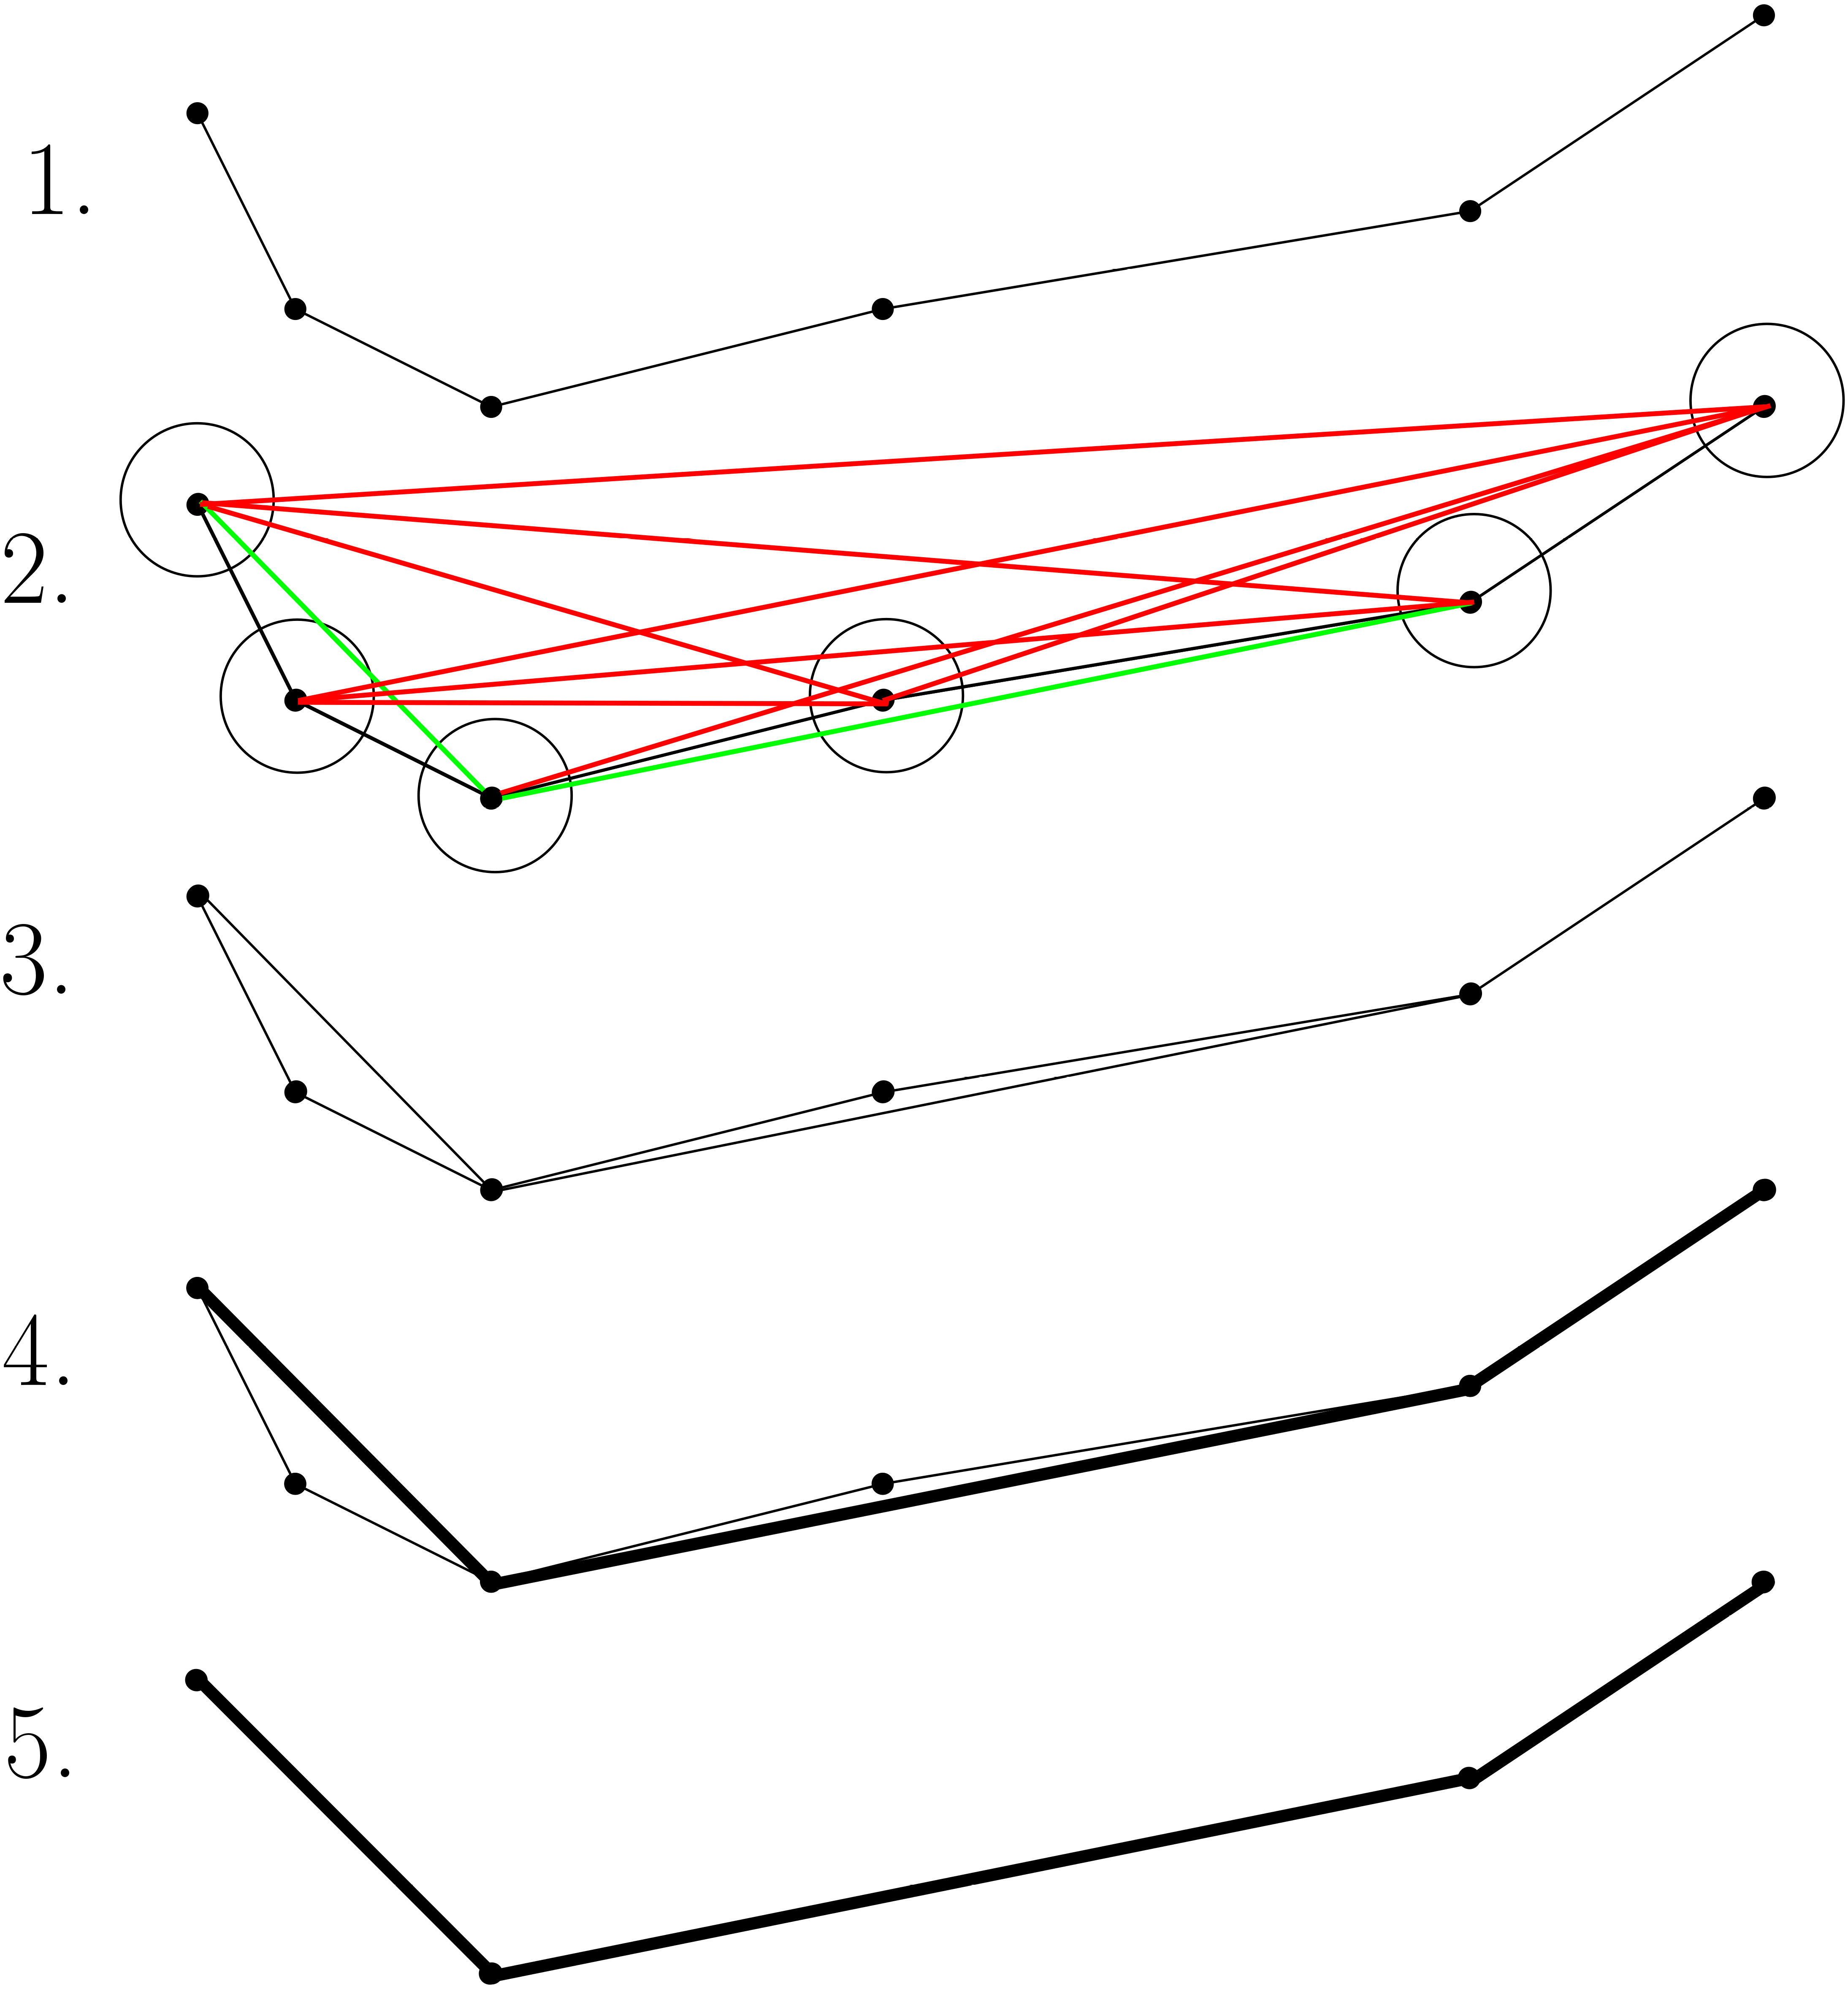
\includegraphics[width=0.5\linewidth]{figures/imaiiri.png}
    \caption[Illustration of Imai-Iri algorithm \cite{van2017extensive}]{Illustration of how the Imai-Iri algorithm generates
    shortcuts. Green lines are allowed shortcuts, red
    lines are not allowed \cite{van2017extensive}.}
    \label{fig:imai}
\end{figure}


\section{Streaming Process Algorithms}

The foundation of traditional data-management systems software is the idea of persistent data sets, which are repeatedly accessed and updated over the course of their existence and are consistently stored in stable storage. Nevertheless, according to \cite{garofalakis2016data}, for a number of developing application domains, data must be processed continuously (24 × 7), without the advantage of multiple passes over a static, persistent data image. Thus, having an algorithm to handle those stream data is crucial.

\subsection{Data Streams}

A sample of the stream's elements can be thought of as the basic description of a data stream. Such a sample has the advantage of being flexible, since it may be further reduced to produce many more data synopses and used as input to a wide range of analytical techniques \cite{garofalakis2016data}. In particular, the sample can serve as a foundation for statistical inference about the contents of the stream if it is obtained by random sampling procedures. In addition to requiring the application of numerous concepts and methods from standard database sampling, data-stream sampling problems also call for important new developments, particularly in handling queries over infinite-length streams. In fact, streaming data's boundless nature marks a significant shift from the conventional environment.  A crucial differentiation is made between a sliding window, where the endpoints advance with time, and a stationary window, where the endpoints are fixed times or locations within the stream sequence. "The most recent n elements in the stream" and "elements that have arrived within the past hour" are two examples of the latter kind of window. In a stationary window, where the initial and last stream items match to the window boundaries, sampling from a finite stream is a specific type of window sampling. Many conventional tools and approaches for database sampling can be simply applied when working with a stationary window. Sliding window sampling is generally a significantly harder task than stationary window sampling since, in the former, components need to be taken out of the sample as soon as they expire and it might be challenging to keep a sample large enough.Furthermore, we take into account "generalized" windows, where the stream is made up of a series of transactions that add and remove things from the window; a sliding window represents the unique scenario where items are removed in the same order that they are added.

\subsection{Stream Processing}

Various scenarios, such as a network of sensor nodes, a stock market, a network monitoring system, and so forth, can provide data streams \cite{namiot2015big}. A variety of approaches, including continuous queries, clustering, classification, frequent item mining, outlier and anomaly detection, can be applied to a data stream. According to \cite{Wähner_2014}, a stream processing solution has to deal with particular challenges mainly  :

\begin{itemize}
    \item  Processing massive amounts of streaming events (filter, aggregate, rule, automate, predict, act, monitor, alert)
    \item  Real-time responsiveness 
    \item  Performance and scalability as data volumes increase in size and complexity
    \item  Analytics: Live data discovery and monitoring, continuous query processing, automated alerts and reactions
\end{itemize}


\subsection{Streaming for Line Simplification}
In this section we will discuss the current state of line simplification algorithm/problem in the context of stream processing. The main problematic of this thesis is related to this problem because of that this subject will have a more in depth analysis.

As mentionned in "Streaming algorithms for line simplification" \cite{abam2007streaming}, suppose we are tracking one, or maybe many, moving objects. Each object is equipped with a device that is continuously transmitting its position. Thus we are receiving a stream of data points that describes the path along which the object moves. The goal is to maintain this path for each object. We are interested in the scenario where we are tracking the objects over a very long period of time, as happens for instance when studying the migratory patterns of animals. In this situation it may be undesirable or even impossible to store the complete stream of data points. Instead we have to maintain an approximation of the input path. This leads us to the following problem: we are receiving a (possibly infinite) stream $p0,p1,p2,...$ of points in the plane, and we wish to maintain a simplification (of the part of the path seen so far) that is as close to the original path as possible, while using not more than a given (fixed) amount of available storage.

\paragraph{Formalization}
In this subsection we will formalize the problem of line simplification in a streaming mode based on the article \cite{abam2007streaming}. To be able to state the problem we wish to solve and the results we obtain more precisely, we first introduce some terminology and definitions. Let $p_0, p_1, \ldots$ be the given stream of input points. We use $P(n)$ to denote the path defined by the points $p_0, p_1, \ldots, p_n$ - that is, the path connecting those points in order - and for any two points $p, q$ on the path we use $P(p, q)$ to denote the subpath from $p$ to $q$. For two vertices $p_i, p_j$ we use $P(i, j)$ as a shorthand for $P\left(p_i, p_j\right)$. A segment $p_i p_j$ with $i<j$ is called a link or sometimes a shortcut. Thus $P(n)$ consists of the links $p_{i-1} p_i$ for $0<i \leqslant n$. We assume a function error is given that assigns a non-negative error to each link $p_i p_j$. A $\ell$-simplification of $P(n)$ is a polygonal path $Q:=q_0, q_1, \ldots, q_k, q_{k+1}$ where $k \leqslant \ell$ and $q_0=p_0$ and $q_{k+1}=p_n$, and $q_1, \ldots, q_k$ is a subsequence of $p_1, \ldots, p_{n-1}$. The error of a simplification $Q$ for a given function error, denoted $\operatorname{error}(Q)$, is defined as the maximum error of any of its links.

\paragraph{Evaluation}
Now consider an algorithm $\mathcal{A}:=\mathcal{A}(\ell)$ that maintains an $\ell$-simplification for the input stream $p_0, p_1, \ldots$, for some given $\ell$. Let $Q_{\mathcal{A}}(n)$ denote the simplification that $\mathcal{A}$ produces for the path $P(n)$. Let $\operatorname{Opt}(\ell)$ denote an optimal off-line algorithm that produces an $\ell$-simplification. Thus $\operatorname{error}\left(Q_{O p t(\ell)}(n)\right)$ is the minimum possible error of any $\ell-$ simplification of $P(n)$. We define the quality of $\mathcal{A}$ using the competitive ratio, as is standard for on-line algorithms. We also allow resource augmentation. More precisely, we allow $\mathcal{A}$ to use a $2k$-simplification, but we compare the error of this simplification to $Q_{O p t(k)}(n)$. (This is similar to Agarwal et al. \cite{agarwal2005near} who compare the quality of their solution to the min- $k$ problem for a given maximum error $\delta$ to the optimal value for maximum error $\delta / 2$.) Thus we define the competitive ratio of an algorithm $\mathcal{A}(2 k)$ as 
$$ 
\text { competitive ratio of } \mathcal{A}(2 k):=\max _{n \geqslant 0} \frac{\operatorname{error}\left(Q_{\mathcal{A}(2 k)}(n)\right)}{\operatorname{error}\left(Q_{O p t(k)}(n)\right)}, 
$$
where $\frac{\operatorname{error}\left(Q_{\mathcal{A}(2 k)}(n)\right)}{\operatorname{error}\left(Q_{O p t(k)}(n)\right)}$ is defined as 1 if $\operatorname{error}\left(Q_{\mathcal{A}(2 k)}(n)\right)=$ $\operatorname{error}\left(Q_{O p t(k)}(n)\right)=0$. We say that an algorithm is $c$ competitive if its competitive ratio is at most $c$.

\paragraph{Algorithm}
We will discuss the existing algorithm for the line simplification in a streaming model. In the article \cite{abam2007streaming} they propose the following algorithm. Our algorithm is quite simple. Suppose we have already handled the points $p_0, \ldots, p_n$. (We assume $n>\ell+1$; until that moment we can simply use all points and have zero error.) Let $Q:=q_0, q_1, \ldots, q_{\ell}, q_{\ell+1}$ be the current simplification. Our algorithm will maintain a priority queue $\mathcal{Q}$ that stores the points $q_i$ with $1 \leqslant i \leqslant \ell$, where the priority of a point is the error (as computed by the oracle) of the link $q_{i-1} q_{i+1}$. In other words, the priority of $q_i$ is (an approximation of) the error that is incurred when $q_i$ is removed from the simplification. Now the next point $p_{n+1}$ is handled as follows:

\begin{enumerate}
    \item  Set $q_{\ell+2}:=p_{n+1}$, thus obtaining an $(\ell+1)$-simplification of $P(n+1)$.
    \item  Compute $\operatorname{error}^*\left(q_{\ell} q_{\ell+2}\right)$ and insert $q_{\ell+1}$ into $\mathcal{Q}$ with this error as priority.
    \item  Extract the point $q_s$ with minimum priority from $\mathcal{Q}$; remove $q_s$ from the simplification.
    \item  Update the priorities of $q_{s-1}$ and $q_{s+1}$ in $\mathcal{Q}$.

\end{enumerate}

As we can see the following algorithm is using the error function in order to correct the result in real-time. There is also the paper about SQUISH that state a similar algorithm \cite{muckell2011squish}. An algorithm of simplification algorithm working in a streaming model is called an online algorithm. 




\section{Error Metrics}

In this section we will explain how to compare a trajectory with its simple counterpart in detail. A polyline P, consisting of a sequence of points $\{p_{1},..., p_{n}\}$, is used in this study  \cite{van2017extensive} to describe trajectories. The points pi consist of the longitude, latitude, and sample time-stamp, Xi, Yi, and ti, respectively. The simplified version of a trajectory is called approximation A, which is a subset of P, the polyline of the original trajectory \cite{van2017extensive}. Additionally, Approximation A needs to contain p1 and pn from the original trajectory. In this thesis, the focus is usually on the spatial and spatio-temporal parameters, with the aim of comparing the trajectory with its simplified version.

\subsection{Hausdorff Distance}


The Hausdorff distance is one basic trajectories similarity metric. It's a particularly broad similarity metric that works with any pair of point sets. The directed Hausdorff distance from P to Q is equal to the Euclidean distance between the point in P that is furthest from any point in Q and the point in Q that is closest to that point \cite{kerkhof2022algorithmic} if we have two sets of points P and Q, such as two trajectories if we treat them as polygonal curves and ignore the timestamps. formally defined, we arrive at:

$$\overrightarrow{\mathrm{H}}(P, Q)=\max _{p \in P} \min _{q \in Q} \| p-q \| $$

The maximum of the directed distances in both directions is hence the undirected Hausdorff distance, which is also simply referred to as the Hausdorff distance.

$$\mathrm{H}(P, Q)=\max \{\overrightarrow{\mathrm{H}}(P, Q), \overrightarrow{\mathrm{H}}(Q, P)\} $$


\subsection{Frechet Distance}


One of the measures of trajectory similarity that is frequently used is the Frechet distance. According to this principle, similar curved polygons must not only be close in space, but there must also be some way of parameterising them that allows them to remain close at all times if we traverse them simultaneously \cite{kerkhof2022algorithmic}. Here, proximity is defined as a small Euclidean distance. Paths are represented in the form of polygons and precise instants are not taken into account. For the polygonal curves P and Q, with probes P and Q respectively, the Frechet distance is specified as follows:

$$\mathrm{F}(P, Q)=\inf _{(\sigma, \theta)} \max _{j:[0,1]}\|P(\sigma(j))-Q(\theta(j))\| $$

wherein the continuous non-decreasing functions $\sigma$ and $\theta$ go from [0, 1] to the real intervals [1, n] and [1, m], respectively. This is frequently explained by the following comparison: \\

Let's say a person is out on a dog walk. The owner's path is P, whereas the dog's path is Q. The dog and owner are free to adjust their speed, but they are not allowed to reverse on the trail. The shortest length of leash the dog can have in order to go on this stroll is known as the Frechet distance. The weak Frechet distance is equivalent, but it does not require that $\theta$ and $\sigma$ be non-decreasing. Sticking to the man-walking-dog analogy, the fact implies that, if a shorter leash be necessary, the man and dog are free to go forward and backward across their path. Thus, a lower bound on the (strong) Fréchet distance can be found using the weak Frechet distance between curves. Another variant of the discrete Frechet distance is $0 \leq \sigma (i+1)-\sigma \ (i) \leq 1$ and $0 \leq \theta \ (i + 1)-\theta \ (i) \leq 1$. These discrete functions are $\sigma $ and $\theta $, and they extend from {0,..., k} to {1,..., n} and {1,...,m}. It has been explained as if someone were walking a pet frog, and the frog could only hop from vertex to vertex, rather than going along the borders of the polygonal curve.An upper bound on the (continuous) Frechet distance between two curves can be found using the discrete Frechet distance between them. It is not entirely simple to calculate the precise Frechet distance between two curves, as one might expect.  A method for calculating this distance was described by Alt and Godau \cite{AltGodau}. They provide a technique for resolving the distance computation problem's decision variation. If the Frechet distance between two curves is at most some number $ \delta $, then this algorithm can provide an answer. They then $ \sigma $ find the lowest value of $ \delta $ using a method known as parametric search. The way their decision method operates is by creating a free space diagram for a given value of $\delta $. It is composed of a grid of $ \times (m - 1) \times (n - 1)$ cells, each of which represents a pair of line segments drawn from P and Q. Every row of cells represents an edge of Q, while every column represents an edge of P. The probe obtained by linearly interpolating between P's second and third probes with a $\lambda$ of 0.6 and the probe obtained by linearly interpolating between Q's third and fourth probes with a $\lambda$ of 0.5, for instance, correspond to the point (2.6, 3.5) in a free space diagram. There are two sections in every cell: banned and free. A point is in the free space if the Euclidean distance between the curves there is less than or equal to $ \delta $. The point is in the prohibited space if the distance is larger than $\delta$. Refer to Figure \ref{fig:fsd} .


\begin{figure}[!ht]
	\centering
	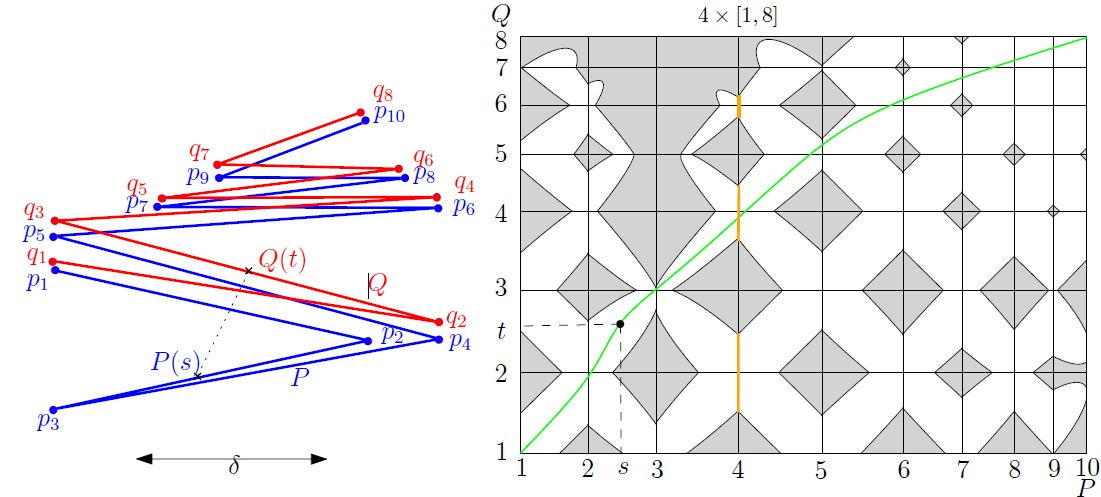
\includegraphics[width=1.0\linewidth]{figures/Figure.jpg}
	\caption[Polygonal curves P and Q's free space diagram for a certain $\delta$]{Polygonal curves P and Q's free space diagram for a certain $\delta$
 %The gray area represents the banned zone, and the white area represents the free space. One edge of P and one edge of Q together correspond to each cell in the FSD. The diagram's free point (s, t) is located on a path that can be reached inside the free space. In the FSD and on the corresponding areas on P and Q, there is a single green spot highlighted. The green path, which is a monotone path in both x and y directions within the free space from (1, 1) to (8, 10), corresponds to parametrizations of P and Q that achieve a maximum Frechet distance of $ \delta $ \cite{kerkhof2022algorithmic}.
 }
	\label{fig:fsd}
\end{figure}
\vspace{1cm}
Now, an x- and y-monotone path from the point (1, 1) to (n,m) entirely through the free space corresponds to parametrizations of P and Q such that the distance between the two is at most $ \delta $  at any time, i.e. the Fréchet distance is at most $ \delta $ . For additional details we refer to the paper by Alt and Godau \cite{AltGodau}.

\subsection{Temporal Integral}
One of the metrics used is the temporal integral. It refers to the integral of the temporal distance between two trajectories over time. Mathematically, if \( P(t) \) and \( Q(t) \) are two trajectories over time \( t \), the temporal integral \( T \) can be expressed as:

\[ T = \int_{t_0}^{t_1} \left( \int_{t_0}^{t} d(P(s), Q(s)) \, ds \right) dt \]

This metric provides information about the temporal gap and can be useful for simplification cases where path Q is derived from path P.


\subsection{Dynamic Time Warping Distance}

Dynamic Time Warping (DTW) is a technique used to find the optimal alignment between two sequences, taking into account the time dimension. This technique is particularly useful for comparing time-dependent sequences that may vary in speed or have local time shifts. The DTW distance is expressed as the minimum cost of a warping path \( p \) between two sequences \( X \) and \( Y \), where \( X \) and \( Y \) are time-dependent sequences \cite{muller2007dynamic}.

To formally define DTW, consider two sequences \( X = (x_1, x_2, \ldots, x_N) \) and \( Y = (y_1, y_2, \ldots, y_M) \) of lengths \( N \) and \( M \) respectively. The goal is to align these sequences in a way that minimizes the overall cost, where the cost is determined by a local cost measure \( c(x, y) \). This local cost measure \( c: F \times F \rightarrow \mathbb{R}_{\geq 0} \) typically assigns a low cost if \( x \) and \( y \) are similar and a high cost if they are different.

The cost matrix \( C \) is constructed by evaluating the local cost measure for each pair of elements from \( X \) and \( Y \), defined as \( C(n, m) = c(x_n, y_m) \). The aim is to find a warping path \( p = (p_1, p_2, \ldots, p_L) \) that aligns \( X \) and \( Y \) with minimal total cost. A warping path must satisfy the following conditions:

\begin{itemize}
    \item \textbf{Boundary Condition}: The path starts at the beginning of both sequences and ends at the end of both sequences, i.e., \( p_1 = (1, 1) \) and \( p_L = (N, M) \).
    \item \textbf{Monotonicity Condition}: The indices of the path must be non-decreasing, i.e., if \( p_{\ell} = (n, m) \) and \( p_{\ell+1} = (n', m') \), then \( n \leq n' \) and \( m \leq m' \).
    \item \textbf{Step Size Condition}: The path can only move in steps of size \( (1, 0) \), \( (0, 1) \), or \( (1, 1) \), ensuring continuity without omitting any elements, i.e., \( p_{\ell+1} - p_{\ell} \in \{(1, 0), (0, 1), (1, 1)\} \).
\end{itemize}

The total cost \( c_p(X, Y) \) of a warping path \( p \) is the sum of the local costs along the path:
\[ c_p(X, Y) = \sum_{\ell=1}^{L} c(x_{n_\ell}, y_{m_\ell}) \]

The DTW distance \( \text{DTW}(X, Y) \) is defined as the total cost of the optimal warping path \( p^* \):
\[ \text{DTW}(X, Y) = c_{p^*}(X, Y) = \min \{ c_p(X, Y) \mid p \text{ is a warping path} \} \]

To compute the DTW distance efficiently, a dynamic programming approach is used. The accumulated cost matrix \( D \) is defined as:
\[ D(n, m) = \text{DTW}(X_{1:n}, Y_{1:m}) \]
where \( X_{1:n} \) and \( Y_{1:m} \) are the prefix sequences of \( X \) and \( Y \).

The recursive formula for computing \( D \) is:
\[ D(n, m) = c(x_n, y_m) + \min \{ D(n-1, m-1), D(n-1, m), D(n, m-1) \} \]

The initialization is as follows:
\[ D(n, 1) = \sum_{k=1}^{n} c(x_k, y_1) \]
\[ D(1, m) = \sum_{k=1}^{m} c(x_1, y_k) \]

The final DTW distance is given by \( D(N, M) \).The dynamic programming algorithm ensures that the computational complexity is \( O(NM) \), making it feasible for practical applications. This approach enables the alignment of sequences even when they are of different lengths or exhibit time distortions.

\begin{figure}[!ht]
	\centering
	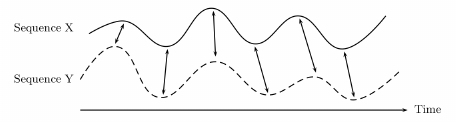
\includegraphics[width=1.0\linewidth]{figures/dtw.png}
	\caption{Two time-dependent sequences aligned in time. The arrows point to aligned points.}
	\label{fig:dtw}
\end{figure}

Figure \ref{fig:dtw} illustrates an example of DTW alignment between two sequences. Sequence \( X \) and Sequence \( Y \) are aligned in such a way that similar patterns in the sequences are matched, despite local time shifts and variations in speed. The arrows in the figure demonstrate the warping path that optimally aligns the sequences, showing how DTW adjusts for temporal distortions to achieve the best match.


